\subsubsection{UC1 - Autenticazione}\label{UC1}

\begin{figure}[H]
  \centering
  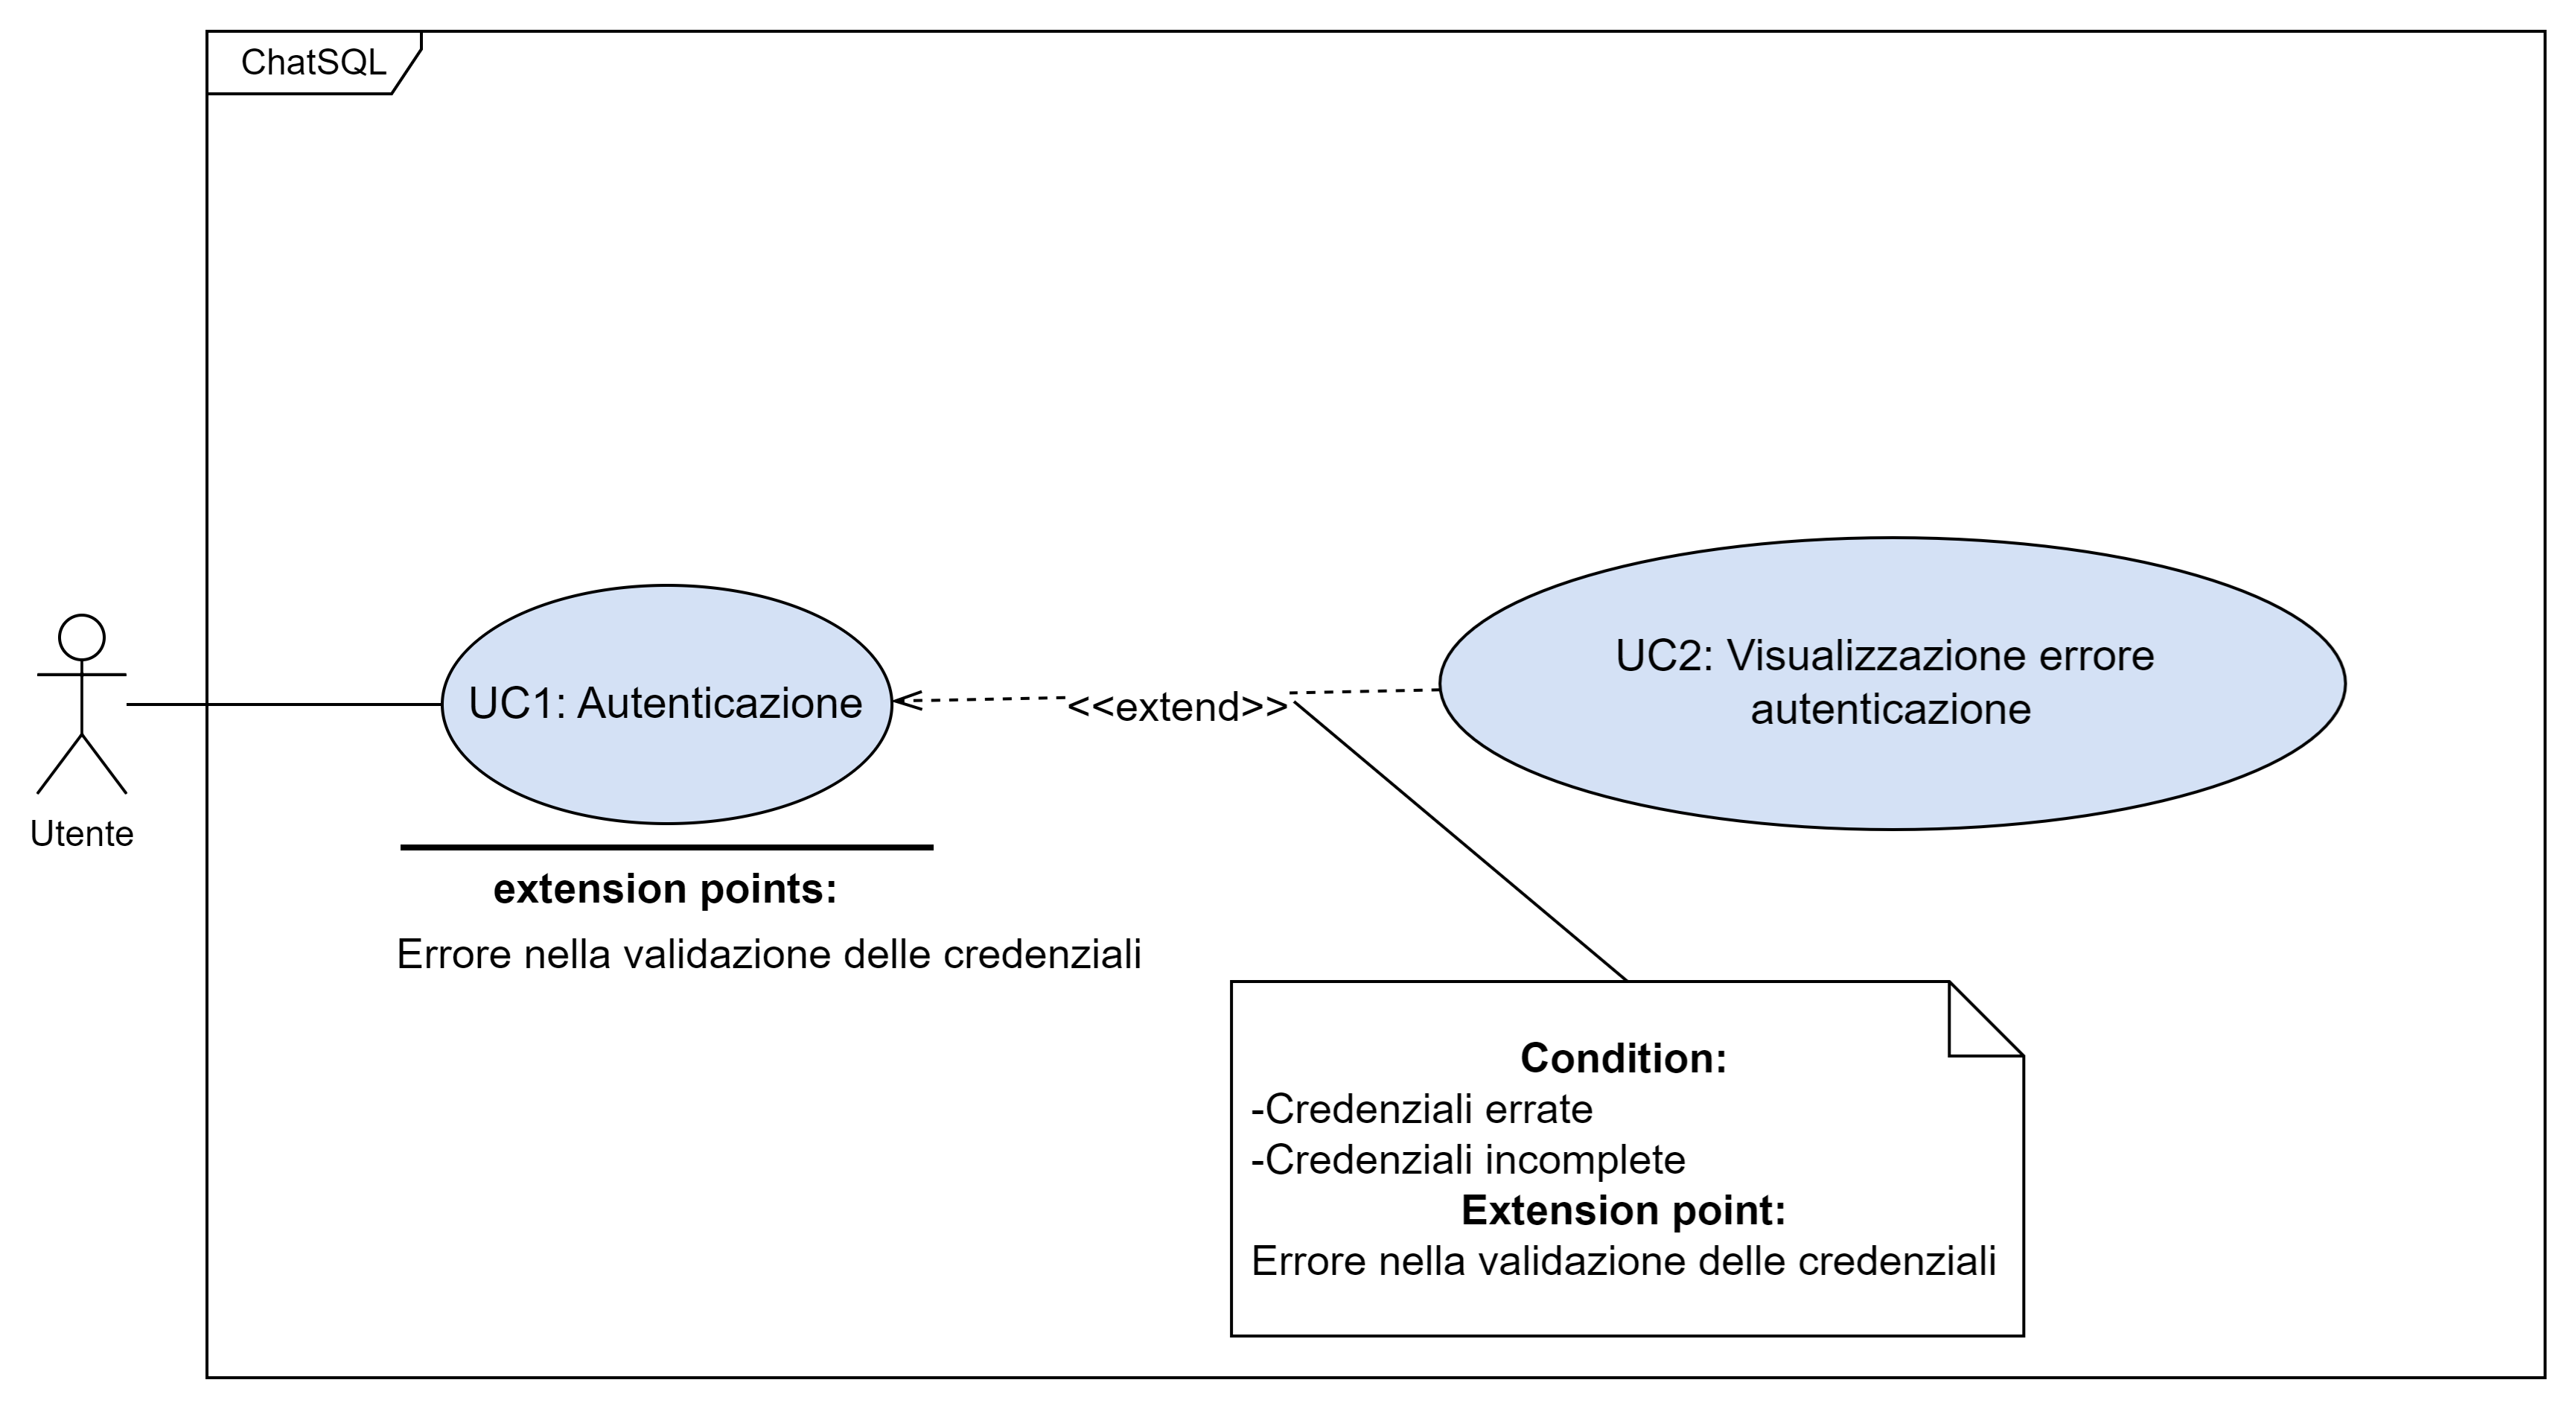
\includegraphics[width=0.90\textwidth]{assets/uc1.png}
  \caption{UC1}
\end{figure}

\paragraph*{Descrizione}
L'autenticazione corrisponde al processo di login, tramite il quale l'Utente può passare alla schermata del Tecnico e ampliare le funzionalità disponibili.

\paragraph*{Attori principali}
Utente

\paragraph*{Precondizioni}
\begin{itemize}
  \item Il sistema è attivo e funzionante;
  \item L'Utente non è autenticato nella sessione corrente.
\end{itemize}

\paragraph*{Postcondizioni}
\begin{itemize}
  \item La procedura di autenticazione si è conclusa con successo;
  \item L'Utente acquisisce il ruolo di tecnico;
  \item Il Tecnico visualizza le funzionalità aggiuntive nell'interfaccia.  
\end{itemize}

\paragraph*{Trigger}
L'Utente desidera accedere all'area riservata al Tecnico.

\paragraph*{Scenario principale}
\begin{itemize}
  \item L'Utente seleziona l'opzione "Login";
  \item L'Utente inserisce le proprie credenziali;
  \item L'Utente effettua l'accesso;
  \item Il sistema mostra le funzionalità disponibili per il Tecnico.
\end{itemize}

\paragraph*{Scenario alternativo}
\begin{enumerate}
  \item Il sistema riscontra un errore durante la validazione delle credenziali (\hyperref[UC2]{UC2});
  \item Viene visualizzato un messaggio con i dettagli dell'errore.
\end{enumerate}

\paragraph*{Estensioni}
\begin{itemize}
  \item Visualizzazione errore autenticazione (\hyperref[UC2]{UC2}).
  \begin{itemize}
    \item Extension point: Errore nella validazione delle credenziali;
    \item Condition: Credenziali errate, credenziali incomplete.
  \end{itemize}
\end{itemize}

% al posto dell'inclusione forse basta il sottocaso d'uso
\paragraph*{Inclusioni}
\begin{itemize}
  \item Inserimento username (\hyperref[UC1point1]{UC1.1});
  \item Inserimento password (\hyperref[UC1point2]{UC1.2}).
\end{itemize}

%%%%%%%%%%%%%%%%%%%%%%%%%%%%%%%%%%%%%%%%%%%%%%%%%%%%%%%%%%%%%%%%%%%%%%%%%%%%%%

\subsubsection{UC1.1 - Inserimento username}\label{UC1point1}

\paragraph*{Descrizione}
La procedura di "inserimento username" corrisponde all'immissione del nome utente nella sezione apposita di login.

\paragraph*{Attori principali}
Utente

\paragraph*{Precondizioni}
\begin{itemize}
  \item Il sistema è attivo e funzionante;
  \item L'Utente ha avviato la procedura di autenticazione (\hyperref[UC1]{UC1}).  
\end{itemize}

\paragraph*{Postcondizioni}
\begin{itemize}
  \item Il nome utente è stato inserito nel campo apposito.
\end{itemize}

\paragraph*{Trigger}
L'Utente desidera inserire il proprio username per accedere alle funzionalità del tecnico.

\paragraph*{Scenario principale}
\begin{enumerate}
  \item L'utente inserisce il proprio username come parte del processo di autenticazione.
\end{enumerate}

%%%%%%%%%%%%%%%%%%%%%%%%%%%%%%%%%%%%%%%%%%%%%%%%%%%%%%%%%%%%%%%%%%%%%%%%%%%%%%

\subsubsection{UC1.2 - Inserimento password}\label{UC1point2}
\paragraph*{Descrizione}
La procedura di "inserimento password" corrisponde all'immissione della password nella sezione apposita di login.

\paragraph*{Attori principali}
Utente

\paragraph*{Precondizioni}
\begin{itemize}
  \item Il sistema è attivo e funzionante;
  \item L'Utente ha avviato la procedura di autenticazione (\hyperref[UC1]{UC1}). 
\end{itemize}

\paragraph*{Postcondizioni}
\begin{itemize}
  \item La password è stata inserita nel campo apposito.
\end{itemize}

\paragraph*{Trigger}
L'Utente vuole inserire la propria password per accedere alle funzionalità del tecnico.

\paragraph*{Scenario principale}
\begin{enumerate}
  \item L'Utente inserisce la propria password come parte del processo di autenticazione.
\end{enumerate}